\documentclass[12pt,a4paper]{article}

\usepackage[utf8]{inputenc}
\usepackage[french]{babel}
\usepackage[T1]{fontenc}
\usepackage[margin=2cm]{geometry}
\usepackage{graphicx}
\usepackage{amsmath}
\usepackage{amsthm}
\usepackage{listings}
\usepackage{courier}

\lstset{basicstyle=\footnotesize\ttfamily,breaklines=true}
\lstset{frame=single}
\lstset{language=Scilab}

\usepackage{float}

\setlength{\parindent}{0pt}
\setlength{\parskip}{0.5em}

\title{\textbf{TP2 “MODÉLISER L’ALÉA” \\ SIMULATION DE FILES D'ATTENTE}}
\author{Clément Riu - Louis Trezzini}
\date{29 mai 2017}

\newtheorem{lemme}{Lemme}

\begin{document}

\maketitle

\paragraph*{Question 1.}

\paragraph*{Question 2.}

\paragraph*{Question 3.}

\begin{figure}[H]
	\centering
	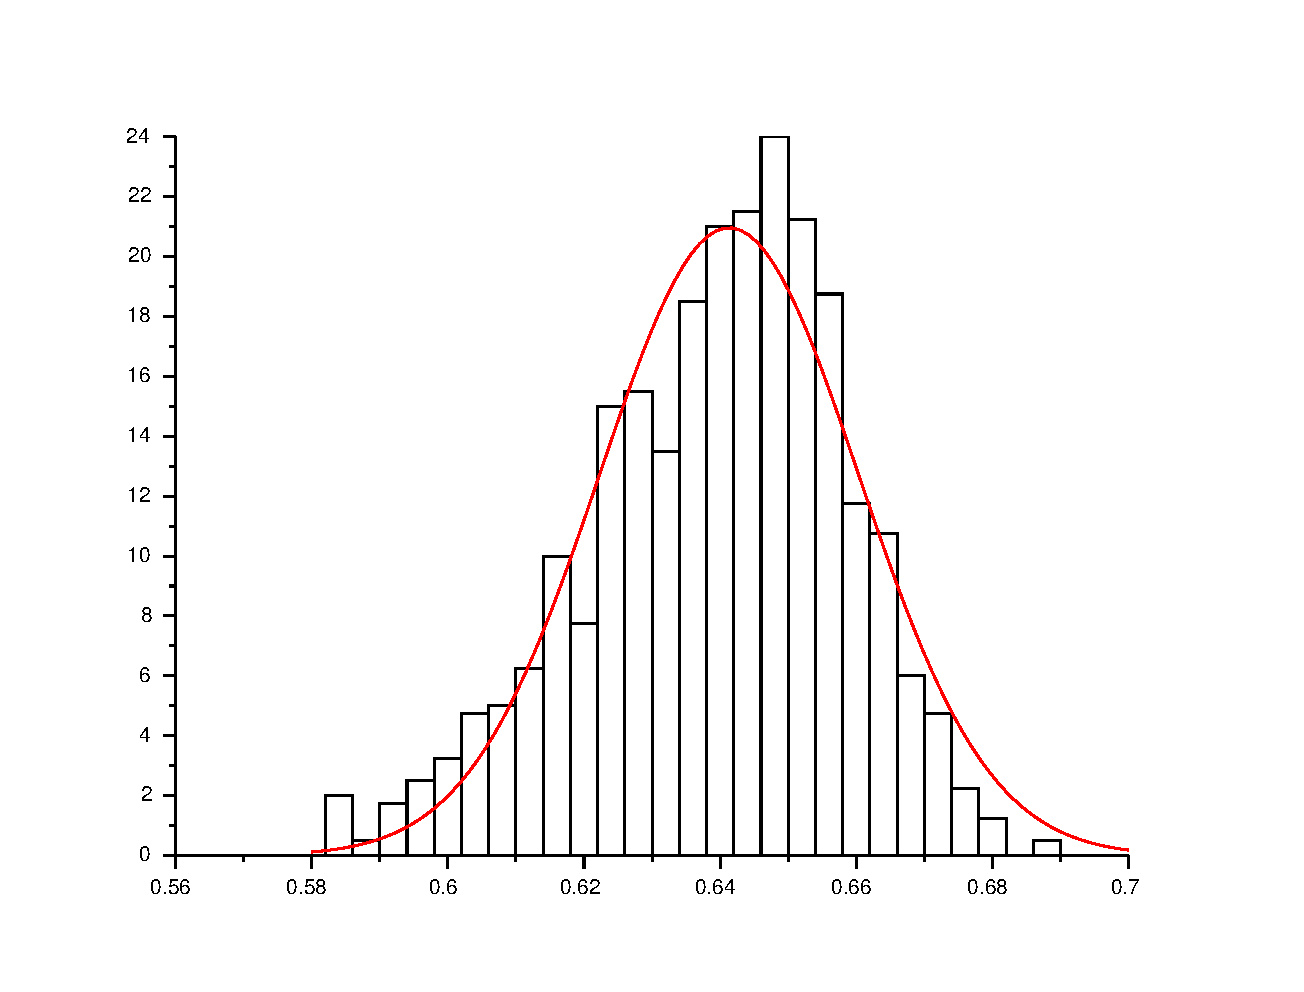
\includegraphics[width=0.95\textwidth]{images/figure0.eps}
	\caption{Loi empirique des données et gaussienne la plus proche.}
\end{figure}

En comparant aux résultats de la page 159 on conclut que le résultat est satisfaisant.
\end{document}
